\chapter{How do people do things}
\begin{flushleft}
	\textit{
		È facile imparare alcune azioni elementari per far funzionare un dispositivo tecnico. Ma cosa succede se le cose non vanno come dovrebbero? Come può l'utente accorgersene, e scoprire cosa fare? }
\end{flushleft}

Per chiarire meglio tutto questo è bene soffermarsi prima sulla psicologia umana e sui modi con cui gli uomini scelgono e valutano le proprie azioni. Fatto ciò si passerà a esaminare il ruolo della cognizione e delle emozioni in tale processo: il piacere quando le cose funzionano senza intoppi e la frustrazione quando le aspettative iniziali degli utenti non sono realizzate.

\section{I Golfi dell'Esecuzione e della Valutazione}
Quando usiamo un oggetto, ci si trova davanti due golfi: il \textbf{golfo dell'esecuzione}, nel quale si cerca di indovinare cosa fare, e il \textbf{golfo della valutazione}, in cui ci si sforza di capire cosa è successo. Il compito del progettista è quello di aiutare gli utenti a superare i due golfi e renderli il meno profondi possibili.

\begin{figure}[!h]
	\centering
	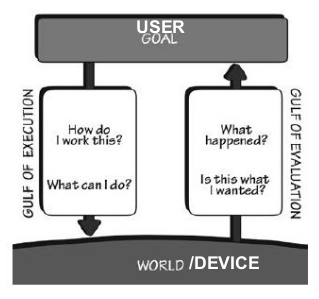
\includegraphics[scale=0.73]{../immagini/Golfi}
	\caption{Golfo dell'esecuzione e golfo della valutazione.}
\end{figure}

Il \textbf{golfo della valutazione} corrisponde allo sforzo necessario per interpretare lo stato fisico del dispositivo e capire fino a che punto sono state realizzate le aspettative e le intenzioni iniziali. Il Golfo è stretto quando il dispositivo fornisce informazioni sul proprio stato, in una forma facile da cogliere e interpretare.

\pagebreak

\begin{flushleft}
	\textit{
		Quali sono gli elementi progettuali più importanti per superare il golfo della valutazione?}
\end{flushleft}

Il \textbf{feedback} e un \textbf{modello concettuale adeguato}.

\begin{flushleft}
	\textit{Quali sono gli elementi progettuali più importanti per superare il golfo dell'esecuzione?}
\end{flushleft}
\textbf{Significanti}, \textbf{constraints}, \textbf{buon mapping} e un modello concettuale adeguato.

Entrambi i golfi sono presenti in molti apparati. Si incontrano spesso difficoltà, puntualmente liquidate accusando sè stessi. Di fronte alle difficoltà nell'uso di congegni che ci si aspetta di saper usare si finisce inevitabilmente col pensare di essere stupidi. Oppure, con dispositivi dall'aspetto più complicato, semplicemente ci si arrende, pensando di essere incapaci di utilizzarli. Queste spiegazioni sono entrambe sbagliate. \textbf{Le difficoltà hanno origine nel design, non nell'utente}.

\section{I sette stadi dell'azione}
Compiere un'azione implica due fasi: \textbf{esecuzione e valutazione degli effetti}, \textbf{fare e interpretare}. Sia l'esecuzione che la valutazione richiedono che si capisca come funziona l'oggetto su cui si applica l'azione e quali risultati essa produce. Entrambe le fasi influiscono sullo stato emotivo dell'utente.

Un progettista deve conciliare il compito che l'utente vorrebbe eseguire e tutte le possibili azioni fisiche che può compiere per eseguirlo. Una volta che l'utente specifica quali azioni compiere, bisogna far in modo le esegua concretamente: ciò costituisce lo \textbf{stadio dell'esecuzione}. \textbf{Identificato il goal, o scopo, l'utente discende attraverso i tre stadi dell'esecuzione: pianificare, specificare ed eseguire.}

\textbf{La valutazione si articola anch'essa in tre stadi: percepire, interpretazione, confrontare.}

Ecco così che si hanno i \textbf{sette stadi dell'azione}: uno per lo scopo, tre per l'esecuzione e tre per la valutazione.
\begin{itemize}
	\item \textbf{Scopo}: definire l'obiettivo.
	\item \textbf{Progettare}: definire l'azione da eseguire.
	\item \textbf{Specificare}: costruire una sequenza d'azione.
	\item \textbf{Eseguire}: eseguire la sequenza specificata.
	\item \textbf{Percepire}: osservare lo stato del mondo.
	\item \textbf{Interpretare}: elaborare la percezione.
	\item \textbf{Confrontare}: rapportare il risultato allo scopo.
\end{itemize}
\begin{center}
	\includegraphics[width=0.5\linewidth]{"../immagini/Sette stadi"}
\end{center}
La maggior parte delle azioni non richiede che si percorrano tutti i sette stadi in sequenza, ma quasi nessuna attività si risolve in tramite un'azione singola.

Di solito si applicano numerose sequenze e l'intera attività può durare ore o giorni. Ci sono molteplici circuiti di feedback, con cui i risultati di un'attività vengono usati per indirizzare l'utente verso altre, in cui uno scopo genera scopi accessori e ogni un progetto sotto-progetti. Ci sono attività in cui lo scopo originario è addirittura dimenticato, scartato o riformulato.

I sette stadi offrono uno schema per sviluppare nuovi prodotti o servizi. I golfi dell'esecuzione e della valutazione sono i punti più ovvi da cui partire, offrendo entrambi spunti per migliorare il prodotto. I progettisti devono svilupparne capacità di osservazione.

\section{Tre livelli di Processing}
Gli stadi dell'azione possono essere associati a tre livelli di processing mentale: viscerale, comportamentale e riflessivo.

\begin{itemize}
	\item \textbf{Livello viscerale}: è il livello più elementare, permette di rispondere prontamente in maniera subconscia, senza consapevolezza o controllo cosciente.
	\item \textbf{Livello comportamentale}: è la sede delle abilità apprese durante circostanze più o meno simili a quelle attuali. Durante l'esecuzione, il livello comportamentale è guidato dalle aspettative, e durante l'attesa di conferma di tali aspettative è invece guidato dalle emozioni. Il livello comportamentale stabilisce in che modo si compie una determinata azione e in che modo si interpreta un determinato feedback.
	\item \textbf{Livello riflessivo}: è il livello della cognizione conscia, è qui che si sviluppa la comprensione profonda e hanno luogo il ragionamento e i processi decisionali. Qui fanno capo i livelli più alti di emotività: soddisfazione e orgoglio, ma anche frustrazione e senso di colpa.
\end{itemize}

\begin{figure}[!h]
	\centering
	\includegraphics[scale=1]{"../immagini/Livelli di Processing"}
\end{figure}

\pagebreak

\textbf{Veicolare informazioni all'utente mentre egli si trova nel livello riflessivo è estremamente efficace}. Al livello riflessivo il suo pensiero è conscio e le emozioni che egli produce sono le più durature.

Gli stimoli riflessivi sono parte integrante del ricordo degli eventi, è importante quindi creare nell'utente ricordi positivi mentre egli è in questo stadio dell'azione, perché tali ricordi sono i più duraturi.

Inoltre è la riflessione, intesa come pensiero cosciente, che induce a consigliare un prodotto e raccomandarne l'uso o magari a sconsigliarlo.

I tre livelli di elaborazione contribuiscono tutti insieme a determinare lo stato emotivo e cognitivo dell'utente. Funzioni riflessive di alto livello possono mettere in moto emozioni più elementari e  queste, a loro volta, possono stimolare attività cognitive di tipo riflessivo.

\section{I sette Principi Fondamentali della Progettazione}
Il modello a sette stadi del ciclo d'azione è un prezioso sussidio per il design, in quanto introduce una lista di domande fondamentali. In generale, ogni stadio dell'azione richiede specifiche strategie progettuali, e, viceversa, presenta occasioni proprie di disastro.

Ne derivano dunque sette domande, a cui dovrebbe poter rispondere chiunque stia usando un determinato prodotto.

\begin{itemize}
	\item \textbf{Cosa voglio ottenere?}
	\item \textbf{Quali sono le sequenze d'azione alternative?}
	\item \textbf{Quale azione posso fare ora?}
	\item \textbf{Come faccio questa azione?}
	\item \textbf{Cosa è successo?}
	\item \textbf{Cosa significa?}
	\item \textbf{Va bene? Ho realizzato il mio scopo?}
\end{itemize}

\begin{figure}[!h]
	\centering
	\includegraphics[scale=0.55]{"../immagini/Sette Domande"}
\end{figure}

\pagebreak

Il progettista ha la responsabilità di garantire che a ogni stadio dell'azione il prodotto fornisca l'informazione necessaria per proseguire correttamente.

L'informazione che serve a rispondere alle domande nelle fasi attuative è definita come \textbf{feedforward}.

L'informazione che aiuta a capire quello che è successo nella fasi percettive è definita invece come \textbf{feedback}.

Il \textbf{feedforward} si realizza mediante l'uso opportuno di significanti, vincoli e mapping, anche il modello concettuale ha un ruolo importante.

Il \textbf{feedback} è dato dall'immediato cambiamento di stato che il prodotto deve mostrare all'utente e, anche qui, una parte importante è svolta dal modello concettuale.

Sia il \textbf{feedback}, che il \textbf{feedforward} devono presentarsi in una forma facilmente interpretabile da chi utilizza il sistema. La presentazione deve corrispondere alla visione che le persone hanno dello scopo che vogliono realizzare e alle loro aspettative. L'informazione erogata deve essere immediatamente comprensibile.

Dalle risposte relative ai sette stadi dell'azione si ricavano sette principi fondamentali del design:

\begin{itemize}
	\item \textbf{Visibilità}: è bene che sia facile scoprire immediatamente quali azioni sono possibili e qual è lo stato attuale del dispositivo.
	\item \textbf{Feedback}: è opportuno che ci sia un'informazione completa e continua riguardo ai risultati delle azioni e allo stato attuale del prodotto o del servizio. Dopo aver eseguito un'azione, deve essere facile determinare il risultato.
	\item \textbf{Modello Concettuale}: il design dovrebbe fornire tutta l'informazione necessaria per creare un buon modello concettuale del sistema, che favorisca la comprensione e la sensazione di controllo da parte dell'utente. Il modello concettuale potenzia sia la visibilità, sia la valutazione dei risultati.
	\item \textbf{Affordance}: è bene che le affordance siano fatte apposta per rendere possibili le azioni desiderate e impossibili quelle indesiderate.
	\item \textbf{Significanti}: un uso efficace dei significanti assicura la visibilità e la comprensibilità dei comandi.
	\item \textbf{Mapping}: è necessario che la relazione fra i comandi e le rispettive azioni obbedisca ai principi del buon mapping, sostenuto, per quanto possibile, dalla disposizione spaziale e dalla contiguità temporale.
	\item \textbf{Vincoli}: bisogna fornire vincoli fisici, logici, semantici e culturali, in modo tale da guidare l'azione e facilitandone l'interpretazione.
\end{itemize}
Questi sette principi sono mappati uno ad uno sugli stadi d'azione dell'utente.

È bene concludere con una nota la parte dedicata a strumenti, metodi ed elementi per il design dello human-computer interaction: per molte attività quotidiane , gli obiettivi e le interazioni non sono ben definiti, \textbf{sono più di tipo opportunistico che frutto di una pianificazione}.

Le azioni opportunistiche sono quelle in cui il comportamento scaturito dalle circostanze prevale sulla pianificazione. Gli utenti in questi casi agiscono in maniera non controllata e quindi non prevedibile.

È difficile fare buon design per queste situazioni, anche attenendosi a tutti i principi esposti fino ad ora: l'utente che agisce in maniera opportunistica romperà in ogni caso questi schemi.

\pagebreak
